\chapter{数据结构与算法}

\section{算法}

\subsection{算法(Algorithm)}

算法是一个很古老的概念,最早来自数学领域。\\

有一个关于算法的小故事:在很久很久以前,曾经有一个顽皮又聪明的熊孩子,天天在课堂上调皮捣蛋。终于有一天,老师忍无可忍,对熊孩子说:“臭小子,你又调皮啊!今天罚你做加法,算出$ 1 + 2 + 3 + \dots + 9999 + 10000 $累加的结果,算不完不许回家!” \\

老师以为,熊孩子会按部就班地一步一步计算:

\vspace{-1cm}

\begin{align*}
	1 + 2  & = 3  \\
	3 + 3  & = 6  \\
	6 + 4  & = 10 \\
	10 + 5 & = 15 \\
	\dots
\end{align*}

这还不得算到明天天亮?够这小子受的!老师心里幸灾乐祸地想着。谁知仅仅几分钟后……\\

“老师,我算完了!结果是50005000,对不对?”\\

“这,这,这……你小子怎么算得这么快?我读书多,你骗不了我的!”\\

看着老师惊讶的表情,熊孩子微微一笑,讲出了他的计算方法。\\

首先把从1到10000这10000个数字两两分组相加:

\vspace{-1cm}

\begin{align*}
	1 + 10000 & = 10001 \\
	2 + 9999  & = 10001 \\
	3 + 9998  & = 10001 \\
	4 + 9997  & = 10001 \\
	\dots
\end{align*}

一共有$ 10000 \div 2 = 5000 $组,所以1到10000相加的总和可以这样来计算:

$$
	(1 + 10000) \times 10000 \div 2 = 50005000
$$

这个熊孩子就是后来著名的犹太数学家约翰·卡尔·弗里德里希·高斯,而他所采用的这种等差数列求和的方法,被称为高斯算法。\\

算法是解决问题的一种方法或一个过程,是一个由若干运算或指令组成的有穷序列。求解问题的算法可以看作是输入实例与输出之间的函数。\\

算法有5个特点:

\begin{enumerate}
	\item 有穷性(finiteness):算法必须能在执行有限个步骤之后终止。
	\item 确定性(definiteness):算法的每一步骤必须有确切的定义。
	\item 输入项(input):一个算法有0个或多个输入。
	\item 输出项(output):一个算法有一个或多个输出,没有输出的算法是毫无意义的。
	\item 可行性(effectiveness):算法中执行的任何计算步骤都是可以被分解为基本的可执行的操作步。
\end{enumerate}

\vspace{0.5cm}

\subsection{算法描述}

算法是可完成特定任务的一系列步骤,算法的计算过程定义明确,通过一些值作为输入并产生一些值作为输出。\\

流程图(flow chart)是算法的一种图形化表示方式,使用一组预定义的符号来说明如何执行特定任务。

\begin{itemize}
	\item 圆角矩形:开始和结束
	\item 矩形:数据处理
	\item 平行四边形:输入/输出
	\item 菱形:分支判断条件
	\item 流程线:步骤
\end{itemize}

\begin{figure}[H]
	\centering
	\begin{tikzpicture}[node distance=2cm]
		\node (start) [startend] {Start};
		\node (init)   [io, below of=start] {$ i = 0 $, $ sum = 0 $};
		\node (decision)  [decision, below of=init] {$ i \le 100 $?};
		\node (accumulation) [process, below of=decision] {$ sum = sum + i $};
		\node (update) [process, below of=accumulation] {$ i = i + 1 $};
		\node (output) [io, right of=decision, xshift=2.5cm] {print $ sum $};
		\node (end) [startend, below of=update] {End};

		\draw [arrow] (start) -- (init);
		\draw [arrow] (init) -- (decision);
		\draw [arrow] (decision) -- node[anchor=east] {yes } (accumulation);
		\draw [arrow] (accumulation) -- (update);
		\draw [arrow] (update) -- (-3,-8) -- (-3,-4) -- (decision);
		\draw [arrow] (decision) -- node[anchor=south] {no} (output);
		\draw [arrow] (output) |- (end);
	\end{tikzpicture}
	\caption{计算$ \sum_{i=1}^{100} i $的流程图}
\end{figure}

伪代码(pseudocode)是一种非正式的,类似于英语结构的,用于描述模块结构图的语言。使用伪代码的目的是使被描述的算法可以容易地以任何一种编程语言实现。

\begin{algorithm}[H]
	\caption{插入排序}
	\begin{algorithmic}[1]
		\Procedure{insertionSort}{A[0..n-1]}
		\For {j = 2 to n - 1}
		\State key = A[j]
		\State i = j - 1
		\While {i > 0 and A[i] > key}
		\State A[i+1] = A[i]
		\State i = i - 1
		\EndWhile
		\State A[i+1] = key
		\EndFor
		\State \Return A
		\EndProcedure
	\end{algorithmic}
\end{algorithm}

\newpage

\section{算法效率}

\subsection{算法效率}

算法有高效的,也有拙劣的。在高斯的故事中,高斯所用的算法显然是更加高效的算法,它利用等差数列的规律,四两拨千斤,省时省力地求出了最终结果。而老师心中所想的算法,按部就班地一个数一个数进行累加,则是一种低效、笨拙的算法。虽然这种算法也能得到最终结果,但是其计算过程要低效得多。\\

在计算机领域,我们同样会遇到各种高效和拙劣的算法。衡量算法好坏的重要标准有两个:时间复杂度、空间复杂度。\\

让我们来想象一个场景:某一天,小灰和大黄同时加入了同一家公司。老板让他们完成一个需求。一天后,小灰和大黄交付了各自的代码,两人的代码实现的功能差不多。但是,大黄的代码运行一次要花100 ms,占用内存5 MB;小灰的代码运行一次要花100 s,占用内存500 MB。\\

“小灰,收拾东西走人,明天不用来上班了!”\\

小灰虽然也按照老板的要求实现了功能,但他的代码存在两个很严重的问题:运行时间长、占用空间大。\\

算法效率分析指的是算法求解一个问题所需要的时间资源和空间资源。效率可以通过对算法执行基本运算(步数)的数目进行估算,度量一个算法运算时间的三种方式:

\begin{itemize}
	\item 最好情形时间复杂度
	\item 最坏情形时间复杂度
	\item 平均情形时间复杂度
\end{itemize}

最坏情形是任何规模为n的问题实例运行时间的上界,即任何规模为n的实例,其运行时间都不会超过最坏情况的运行时间。\\

对某些算法,最坏情况经常发生。例如在某个数据库中查询不存在的数据就是查询算法的最坏情形。平均情形有时跟最坏情形差不多。\\

\subsection{时间复杂度(Time Complexity)}

算法的效率主要取决于算法本身,与计算模型(计算机)无关,可以通过分析算法的运行时间从而比较出算法之间的快慢。分析算法的运行时间应该主要关注与问题规模有关的主要项,其它低阶项,甚至主要项的常数系数都可以忽略。\\

渐进时间复杂度用大写$ O $来表示,所以也被称为大$ O $表示法。\\

时间复杂度有如下原则:

\begin{enumerate}
	\item 如果运行时间是常数量级,则用$ O(1) $表示。
	\item 只保留时间函数中的最高阶项。
	\item 如果最高阶项存在,则省去最高阶项前面的系数。
\end{enumerate}

在编程的世界中有各种各样的算法,有许多不同形式的时间复杂度,例如:$ O(1) $、$ O(logn) $、$ O(n) $、$ O(nlogn) $、$ O(n^2) $、$ O(2^n) $、$ O(n!) $等。\\

\subsection{空间复杂度(Space Complexity)}

内存空间是有限的,在时间复杂度相同的情况下,算法占用的内存空间自然是越小越好。如何描述一个算法占用的内存空间的大小呢?这就用到了算法的另一个重要指标——空间复杂度。\\

和时间复杂度类似,空间复杂度是对一个算法在运行过程中临时占用存储空间大小的量度,它同样使用了大$ O $表示法。\\

正所谓鱼和熊掌不可兼得,很多时候,我们不得不在时间复杂度和空间复杂度之间进行取舍。在绝大多数时候,时间复杂度更为重要一些,我们宁可多分配一些内存空间,也要提升程序的执行速度。

\newpage

\section{基础算法}

\subsection{暴力枚举}

暴力破解法也称穷举法,思想就是列举出所有可能情况,然后根据条件判断此答案是否合适,合适就保留,不合适就丢弃。暴力法主要利用计算机运算速度快、精确度高的特点。因此暴力法是通过牺牲时间来换取答案的全面性。\\

\mybox{鸡兔同笼}\\

上有三十五头,下有九十四足,问鸡兔各几何?

\begin{lstlisting}[language=C]
void count(int head, int foot) {
	for(int chicken = 0; chicken <= head; chicken++) {
		int rabbit = head - chicken;
		if(chicken*2 + rabbit*4 == foot) {
			printf("鸡:%2d\t兔:%2d\n", chicken, rabbit);
		}
	}
}
\end{lstlisting}

\vspace{0.5cm}

\mybox{百钱买百鸡}\\

公鸡5文钱1只,母鸡3文钱1只,小鸡1文钱3只,如果用100文钱买100只鸡,那么公鸡、母鸡和小鸡各应该买多少只?

\begin{lstlisting}[language=C]
void buy(int n, int money) {
	for(int x = 0; x <= n/5; x++) {
		for(int y = 0; y <= n/3; y++) {
			int z = n - x - y;
			if(z > 0 && z % 3 == 0 && 5*x + 3*y + z/3 == money) {
				printf("公鸡:%3d\t母鸡:%3d\t小鸡:%3d\n", x, y, z);
			}
		}
	}
}
\end{lstlisting}

\vspace{0.5cm}

\subsection{字符串逆序}

将一个字符串中的字符顺序颠倒过来实现逆序。\\

\mybox{字符串逆序}

\begin{lstlisting}[language=C]
void reverse(char *str) {
	int i = 0;
	int j = strlen(str) - 1;
	while(i < j) {
		char temp = str[i];
		str[i] = str[j];
		str[j] = temp;
		i++;
		j--;
	}
}
\end{lstlisting}

\vspace{0.5cm}

\subsection{随机算法}

随机算法就是在算法中引入随机因素,通过随机数选择算法的下一步操作,它采用了一定程序的随机性作为其逻辑的一部分。\\

只有随机数生成器的情况下如何计算圆周率的近似值?蒙特卡洛算法就是一种随机算法,用于近似计算圆周率$ \pi $的值。\\

蒙特卡洛算法是以概率和统计理论方法为基础的一种计算方法,将所求解的问题同一定的概率模型相联系,用电子计算机实现统计模拟或抽样,以获得问题的近似解。为象征性地表明这一方法的概率统计特征,故借用赌城蒙特卡罗命名。\\

蒙特卡洛算法的基本思想就是当样本数量足够大时,可以用频率去估计概率,这也是求圆周率$ \pi $的常用方法。

\begin{figure}[H]
	\centering
	\begin{tikzpicture}
		\draw[fill=gray, opacity=0.1] (\radius,0) arc(0:90:\radius) -- (0,0) -- cycle;
		\draw[gray, opacity=0.25] (0,0) rectangle (\radius,\radius);
		\draw[->] (0,0) -- (1.1*\radius,0);
		\draw[->] (0,0) -- (0,1.1*\radius);
		\foreach \i in {1,2,...,1000}{
				\typeout{Point \i}
				\pgfmathsetmacro\x{\radius*rnd}
				\typeout{X \x}
				\pgfmathsetmacro\y{\radius*rnd}
				\typeout{Y \y}
				\pgfmathsetmacro\k{(pow(\x,2)+pow(\y,2)) <pow(\radius,2)}
				\typeout{im Kreis?: \k}
				\pgfmathparse{ifthenelse(\k==1,"red","blue")}
				\fill[\pgfmathresult] (\x,\y)circle(1pt);
			}
	\end{tikzpicture}
	\caption{蒙特卡洛算法}
\end{figure}

当在$ [0, 1] $的范围内随机选择一个坐标$ (x, y) $时,每个坐标点被选中的概率相等,则坐标落在直径为1的正方形中的圆的概率为:

$$
	P \left( \sqrt{x^2 + y^2} \le 1 \right) = {\pi \over 4}
$$

在生成大量随机点的前提下能得到尽可能接近圆周率的值。\\

\mybox{蒙特卡罗算法}

\begin{lstlisting}[language=C]
double montePI(int n) {
	int cnt = 0;        // 圆内点的数量
	for(int i = 0; i < n; i++) {
		double x = rand() / (RAND_MAX + 1.0);   // [0, 1]
		double y = rand() / (RAND_MAX + 1.0);   // [0, 1]
		if(sqrt(x*x + y*y) <= 1) {
			cnt++;
		}
	}
	return 4.0 * cnt / n;
}
\end{lstlisting}

\newpage

\section{数据结构}

\subsection{数据结构(Data Structure)}

数据结构是算法基石,是计算机数据的组织、管理和存储的方式,数据结构指的是相互之间存在一种或多种特定关系的数据元素的集合。一个好的数据结构可以带来更高的运行或者存储效率。\\

\begin{figure}[H]
	\centering
	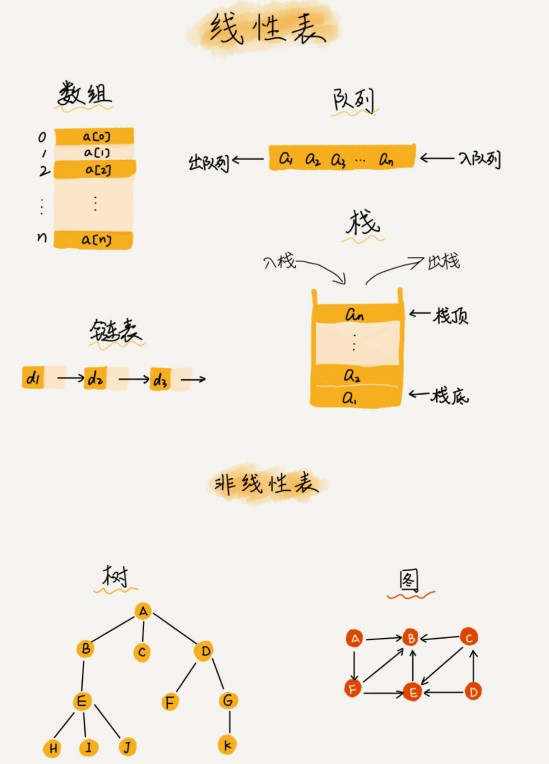
\includegraphics[]{img/C1/1-4/1.png}
	\caption{常用数据结构}
\end{figure}

\newpage